% =====================================================================
% BMED365 (Spring 2027) — Lab 5: The Computational Kiwi Challenge
% Companion Guide (Part 1): Math Primer, Multi-Scale Atlas & Morphogenesis
% Compile with: pdflatex foundations-atlas-and-morphogenesis.tex (run twice)
% =====================================================================
\documentclass[10.5pt,a4paper]{article}

\usepackage[utf8]{inputenc}
\usepackage[T1]{fontenc}
\usepackage[english]{babel}
\usepackage{lmodern}
\usepackage{microtype}
\usepackage{graphicx}
\usepackage{booktabs}
\usepackage{tabularx}
\usepackage{array}
\usepackage{colortbl}
\usepackage{xcolor}
\usepackage{amsmath,amssymb}
\usepackage{enumitem}
\usepackage[margin=1.9cm,headheight=14pt]{geometry}
\usepackage{fancyhdr}
\usepackage{titlesec}
\usepackage[most]{tcolorbox}
\usepackage{listings}
\usepackage{float}
\usepackage{tikz}
\usetikzlibrary{arrows.meta,positioning,shapes.geometric,fit,backgrounds,calc}
\usepackage{hyperref}

% =====================================================================
% COLORS & HYPERREF (UiB / BMED365 House Style)
% =====================================================================
\definecolor{uibblue}{RGB}{0, 61, 115}
\definecolor{uibred}{RGB}{175, 28, 44}
\definecolor{kiwigreen}{RGB}{27, 138, 90}
\definecolor{amberwarn}{RGB}{195, 110, 0}
\definecolor{lightgray}{RGB}{246, 248, 250}
\definecolor{rowalt}{RGB}{242, 246, 251}
\definecolor{codebg}{RGB}{248, 249, 251}
\definecolor{codekw}{RGB}{0, 75, 145}
\definecolor{codestr}{RGB}{155, 35, 45}
\definecolor{codecmt}{RGB}{95, 105, 115}

\hypersetup{
    colorlinks=true,
    linkcolor=uibblue,
    citecolor=uibblue,
    urlcolor=uibred,
    pdftitle={Computational Modeling of the Kiwifruit (Part 1): Math Primer, Multi-Scale Atlas & Morphogenesis (BMED365 Spring 2027)},
    pdfauthor={Arvid Lundervold (UiB / MMIV) -- BMED365 Spring 2027}
}

% =====================================================================
% TYPOGRAPHY, HEADERS & CALLOUT BOXES
% =====================================================================
\setlength{\parindent}{0pt}
\setlength{\parskip}{0.45em}
\setlist[itemize]{topsep=2pt,itemsep=2pt,leftmargin=1.4em}
\setlist[enumerate]{topsep=2pt,itemsep=2pt,leftmargin=1.6em}

\newcolumntype{L}[1]{>{\raggedright\arraybackslash}p{#1}}
\newcolumntype{C}[1]{>{\centering\arraybackslash}p{#1}}
\newcolumntype{R}[1]{>{\raggedleft\arraybackslash}p{#1}}
\newcolumntype{Y}{>{\raggedright\arraybackslash}X}

\titleformat{\section}{\Large\bfseries\color{uibblue}}{\thesection}{0.7em}{}[\vspace{1pt}\titlerule]
\titleformat{\subsection}{\large\bfseries\color{uibblue!88!black}}{\thesubsection}{0.6em}{}
\titleformat{\subsubsection}{\normalsize\bfseries\color{uibblue!75!black}}{\thesubsubsection}{0.5em}{}
\titlespacing*{\section}{0pt}{1.15em}{0.45em}
\titlespacing*{\subsection}{0pt}{0.85em}{0.3em}

\pagestyle{fancy}
\fancyhf{}
\fancyhead[L]{\footnotesize\textcolor{gray}{BMED365 (Spring 2027) $\cdot$ Lab 5: Computational Kiwi Challenge (Part 1)}}
\fancyhead[R]{\footnotesize\textcolor{gray}{Math Primer, Multi-Scale Atlas \& Morphogenesis}}
\fancyfoot[L]{\footnotesize\textcolor{gray}{University of Bergen \& MMIV $\cdot$ CC BY-SA 4.0}}
\fancyfoot[R]{\footnotesize\textcolor{gray}{Page \thepage}}
\renewcommand{\headrulewidth}{0.4pt}
\renewcommand{\footrulewidth}{0.2pt}

\newtcolorbox{infobox}[1][]{
    enhanced,
    colback=lightgray, colframe=uibblue,
    fonttitle=\bfseries\small, title=#1,
    boxrule=0.6pt, arc=2.5pt, left=7pt, right=7pt, top=5pt, bottom=5pt
}

\newtcolorbox{warningbox}[1][]{
    enhanced,
    colback=uibred!4, colframe=uibred,
    fonttitle=\bfseries\small, title=#1,
    boxrule=0.6pt, arc=2.5pt, left=7pt, right=7pt, top=5pt, bottom=5pt
}

\newtcolorbox{qabox}[1][]{
    enhanced,
    colback=kiwigreen!5, colframe=kiwigreen!85!black,
    fonttitle=\bfseries\small, title=#1,
    boxrule=0.6pt, arc=2.5pt, left=7pt, right=7pt, top=5pt, bottom=5pt
}

\lstdefinestyle{pybmed}{
    language=Python,
    backgroundcolor=\color{codebg},
    basicstyle=\ttfamily\scriptsize,
    keywordstyle=\bfseries\color{codekw},
    stringstyle=\color{codestr},
    commentstyle=\itshape\color{codecmt},
    showstringspaces=false,
    breaklines=true,
    breakatwhitespace=true,
    frame=single,
    rulecolor=\color{uibblue!30},
    framesep=4pt,
    xleftmargin=3pt,
    xrightmargin=3pt,
    columns=fullflexible,
    keepspaces=true,
    upquote=true
}

% =====================================================================
% DOCUMENT START
% =====================================================================
\begin{document}

% Title Banner
\begin{tcolorbox}[enhanced, colback=uibblue!6, colframe=uibblue, boxrule=1.0pt, arc=3pt, left=10pt, right=10pt, top=9pt, bottom=9pt]
{\LARGE\bfseries\color{uibblue} Computational Modeling of the Kiwifruit (Part 1)}\\[3pt]
{\normalsize\bfseries Mathematical Primer, Multi-Scale Anatomical \& Physiological Atlas, and Growth \& Morphogenesis}\\[3pt]
{\small \textbf{Course:} BMED365 --- Computational Imaging, Modeling and AI in Biomedicine (Spring 2027), University of Bergen \& MMIV\\
\textbf{Coordinator:} Arvid Lundervold \quad$\cdot$\quad \textbf{Environment:} Pure CPU (\texttt{NumPy}/\texttt{SciPy}/\texttt{nibabel}; \texttt{bmed365-2027} \texttt{uv} \& Google Colab)\\[3pt]
\textbf{Companion Resources:} \href{https://github.com/arvidl/BMED365-2027/blob/main/Lab5-Comp-Mod/Kiwi-challenge/notebooks/00-kiwi-math-primer-for-biomedicine.ipynb}{NB \texttt{00} (Math Primer)} $\;\vert\;$ \href{https://github.com/arvidl/BMED365-2027/blob/main/Lab5-Comp-Mod/Kiwi-challenge/notebooks/00a-kiwi-anatomical-and-physiological-atlas.ipynb}{NB \texttt{00a} (Atlas)} $\;\vert\;$ \href{https://github.com/arvidl/BMED365-2027/blob/main/Lab5-Comp-Mod/Kiwi-challenge/notebooks/01-kiwi-growth-and-morphogenesis.ipynb}{NB \texttt{01} (Morphogenesis)} $\;\vert\;$ \href{https://github.com/arvidl/BMED365-2027/blob/main/Lab5-Comp-Mod/Kiwi-challenge/docs/foundations-atlas-and-morphogenesis.md}{Markdown} $\;\vert\;$ \href{https://github.com/arvidl/BMED365-2027/blob/main/Lab5-Comp-Mod/Kiwi-challenge/docs/inverse-problems-and-digital-twin.pdf}{Part~2 PDF}}
\end{tcolorbox}

\vspace{-2pt}
{\small\tableofcontents}
\vspace{4pt}
\hrule
\vspace{6pt}

% =====================================================================
% SECTION 1: NON-TECHNICAL INTRODUCTION & VISUAL INTUITION
% =====================================================================
\section{A Non-Technical Introduction: Big Ideas, Definitions \& Visual Intuition}

\begin{infobox}[Who This Section Is For (Start Here!)]
Mathematical models in biology papers often look intimidating because authors show only the finished equations while hiding the physical intuition behind them. Before introducing a single derivative or differential equation, this opening section gives a \textbf{plain-English tour} of how we read the kiwifruit's multi-scale anatomy and simulate how living tissue builds a 3D organ --- written for biomedicine and health-science master's students with moderate math background.
\end{infobox}

\subsection{Why ``Mathematize'' a Kiwifruit in a Biomedicine Course?}

In \href{https://github.com/arvidl/BMED365-2027/tree/main/Lab4-Comp-Imag/Kiwi-challenge}{\textbf{Lab 4 (Computational Imaging)}}, we approached our 2005 7\,Tesla MRI scan of an intact \texttt{'Hayward'} kiwifruit the way a radiologist approaches a brain MRI: we asked \textbf{``What is inside?''} --- measuring an $85.97\text{ cm}^3$ fruit containing roughly $1{,}440$ dark seeds.

In \textbf{Lab 5 (Computational Modeling)}, we flip the camera around and ask: \textbf{``How did nature build this 3D organ, and what happens if we perturb the biological rules?''}
\begin{itemize}
    \item Why did the berry stop growing right around $86\text{ cm}^3$, and why does the thickness of each slice track how many seeds sit in that slice?
    \item Why was the scanner's hospital-style DICOM tag \texttt{PatientSex = F} literally true --- how does a single Y-chromosome gene decide whether a flower grows an ovary or remains male?
    \item How does a microscopic ring of cells --- with no ruler and no CAD blueprint --- spontaneously count out \textbf{33 evenly spaced radial seed chambers}?
    \item Why does the bright white central core of a cut kiwifruit turn \textbf{dark} in 7\,T MRI, while the translucent jelly around the seeds shines \textbf{190$\times$ brighter} than the seeds?
\end{itemize}

This is not just botanical trivia. Plants and humans diverged 1.5 billion years ago, yet living tissues in both kingdoms obey the \textbf{exact same physical and mathematical laws}: drug-receptor saturation (clinical pharmacodynamics), bistable genetic sex switches (human \texttt{SRY}/\texttt{SOX9} vs.\ \texttt{WNT4}), fluid-pressure expansion (glomerular filtration, edema, and polycystic kidney cysts), Turing self-organization (how five human fingers space out in an embryonic limb bud), and spin-echo MRI water physics (even extending directly to human clinical gastrointestinal MRI trials of kiwifruit!).

\subsection{Visual Intuition: Four Big Ideas Before Any Equations}

\begin{figure}[H]
\centering
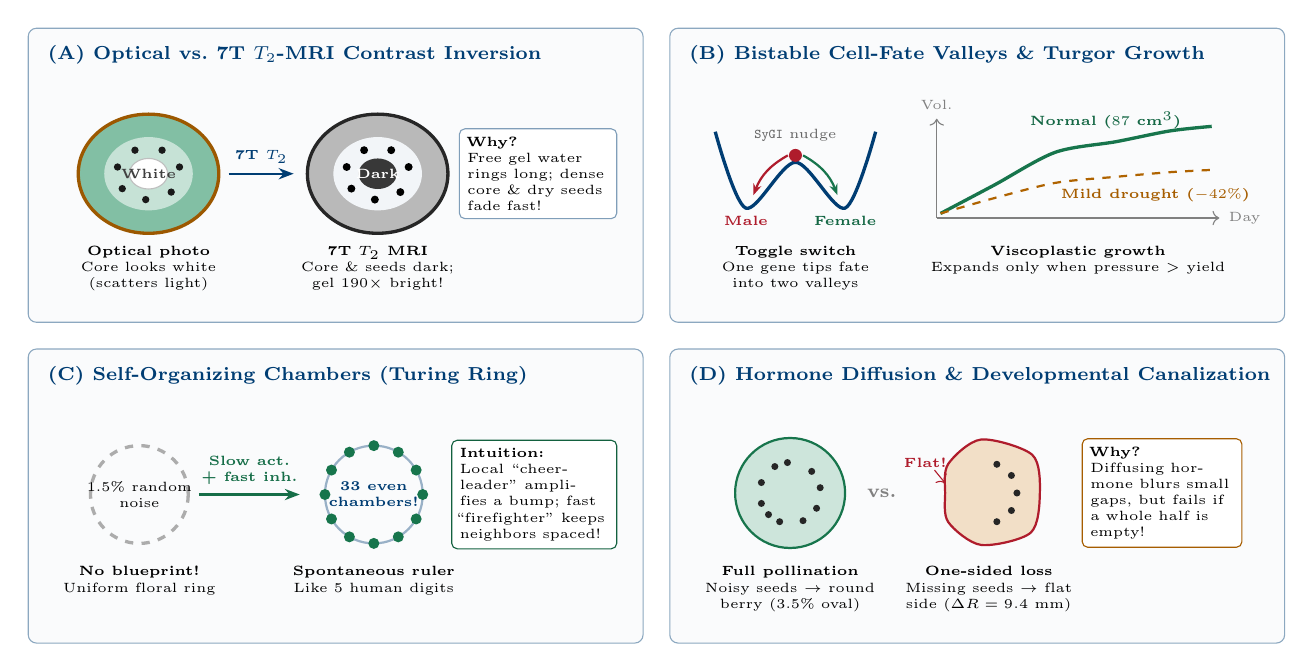
\begin{tikzpicture}[
    scale=0.97, transform shape,
    font=\scriptsize,
    panel/.style={rectangle, rounded corners=3pt, draw=uibblue!45, fill=lightgray!55, inner sep=4pt, minimum width=8.05cm, minimum height=3.85cm}
]
% --- PANEL A: Optical vs 7T T2 Inversion ---
\node[panel] (pA) at (0,0) {};
\node[anchor=north west, font=\scriptsize\bfseries\color{uibblue}] at ([xshift=4pt,yshift=-3pt]pA.north west) {(A) Optical vs.\ 7T $T_2$-MRI Contrast Inversion};

\begin{scope}[shift={(-3.55,-1.08)}]
    % Optical kiwi
    \fill[kiwigreen!55, draw=amberwarn!80!black, very thick] (1.10,1.10) ellipse (0.92 and 0.78);
    \fill[kiwigreen!25] (1.10,1.10) ellipse (0.58 and 0.48);
    \fill[white, draw=gray!50] (1.10,1.10) ellipse (0.25 and 0.20);
    \foreach \ang in {15,65,115,165,215,265,315}{
        \fill[black!90] ({1.10+0.42*cos(\ang)},{1.10+0.34*sin(\ang)}) circle (0.048);
    }
    \node[font=\tiny\bfseries, color=black!75] at (1.10,1.10) {White};
    \node[below, align=center, font=\tiny] at (1.10,0.28) {\textbf{Optical photo}\\Core looks white\\(scatters light)};

    \draw[-{Stealth[length=1.9mm]}, thick, color=uibblue] (2.15,1.10) -- (3.00,1.10) node[midway, above, font=\tiny\bfseries\color{uibblue}] {7T $T_2$};

    % MRI kiwi
    \fill[gray!55, draw=black!85, very thick] (4.10,1.10) ellipse (0.92 and 0.78);
    \fill[white!95!uibblue] (4.10,1.10) ellipse (0.58 and 0.48);
    \fill[black!78] (4.10,1.10) ellipse (0.25 and 0.20);
    \foreach \ang in {15,65,115,165,215,265,315}{
        \fill[black] ({4.10+0.42*cos(\ang)},{1.10+0.34*sin(\ang)}) circle (0.052);
    }
    \node[font=\tiny\bfseries, color=white] at (4.10,1.10) {Dark};
    \node[below, align=center, font=\tiny] at (4.10,0.28) {\textbf{7T $T_2$ MRI}\\Core \& seeds dark;\\gel $190\times$ bright!};

    % Mini note
    \node[rectangle, rounded corners=2pt, draw=uibblue!50, fill=white, align=left, font=\tiny, text width=1.85cm, inner sep=3pt] at (6.20,1.10) {\textbf{Why?}\\Free gel water rings long; dense core \& dry seeds fade fast!};
\end{scope}

% --- PANEL B: Bistable Switch & Turgor Balloon ---
\node[panel] (pB) at (8.40,0) {};
\node[anchor=north west, font=\scriptsize\bfseries\color{uibblue}] at ([xshift=4pt,yshift=-3pt]pB.north west) {(B) Bistable Cell-Fate Valleys \& Turgor Growth};

\begin{scope}[shift={(4.82,-1.08)}]
    % Waddington two-valley curve
    \draw[uibblue, very thick] plot[smooth] coordinates {(0.15,1.65) (0.55,0.65) (1.20,1.25) (1.85,0.65) (2.25,1.65)};
    \fill[uibred] (1.20,1.34) circle (0.085);
    \draw[-{Stealth[length=1.4mm]}, thick, color=uibred] (1.10,1.34) to[bend right=20] (0.65,0.82);
    \draw[-{Stealth[length=1.4mm]}, thick, color=kiwigreen!85!black] (1.30,1.34) to[bend left=20] (1.75,0.82);
    \node[font=\tiny\bfseries, color=uibred] at (0.55,0.48) {Male};
    \node[font=\tiny\bfseries, color=kiwigreen!75!black] at (1.85,0.48) {Female};
    \node[font=\tiny, color=gray!80!black] at (1.20,1.60) {\texttt{SyGI} nudge};
    \node[below, align=center, font=\tiny] at (1.20,0.28) {\textbf{Toggle switch}\\One gene tips fate\\into two valleys};

    % Lockhart pressure gauge
    \draw[->, thin, gray] (3.05,0.52) -- (6.75,0.52) node[right, font=\tiny] {Day};
    \draw[->, thin, gray] (3.05,0.52) -- (3.05,1.82) node[above, font=\tiny] {Vol.};
    \draw[kiwigreen!85!black, very thick] plot[smooth] coordinates {(3.10,0.58) (3.80,0.95) (4.60,1.38) (5.40,1.52) (6.10,1.66) (6.65,1.72)};
    \draw[amberwarn!90!black, thick, dashed] plot[smooth] coordinates {(3.10,0.58) (3.80,0.78) (4.60,0.98) (5.40,1.06) (6.10,1.12) (6.65,1.15)};
    \node[font=\tiny\bfseries, color=kiwigreen!75!black, anchor=west] at (4.15,1.80) {Normal ($87\text{ cm}^3$)};
    \node[font=\tiny\bfseries, color=amberwarn!85!black, anchor=west] at (4.55,0.82) {Mild drought ($-42\%$)};
    \node[below, align=center, font=\tiny] at (4.90,0.28) {\textbf{Viscoplastic growth}\\Expands only when pressure $>$ yield};
\end{scope}

% --- PANEL C: Turing Cheerleader + Firefighter ---
\node[panel] (pC) at (0,-4.20) {};
\node[anchor=north west, font=\scriptsize\bfseries\color{uibblue}] at ([xshift=4pt,yshift=-3pt]pC.north west) {(C) Self-Organizing Chambers (Turing Ring)};

\begin{scope}[shift={(-3.55,-5.28)}]
    % Flat noisy ring
    \draw[gray!65, very thick, dashed] (0.98,1.10) circle (0.64);
    \node[font=\tiny, align=center] at (0.98,1.10) {1.5\% random\\noise};
    \node[below, align=center, font=\tiny] at (0.98,0.28) {\textbf{No blueprint!}\\Uniform floral ring};

    \draw[-{Stealth[length=1.9mm]}, thick, color=kiwigreen!80!black] (1.76,1.10) -- (3.08,1.10) node[midway, above, align=center, font=\tiny\bfseries\color{kiwigreen!75!black}] {Slow act.\\+ fast inh.};

    % Patterned ring with radial peaks
    \draw[uibblue!40, thick] (4.05,1.10) circle (0.64);
    \foreach \k in {0,30,60,90,120,150,180,210,240,270,300,330}{
        \fill[kiwigreen!85!black] ({4.05+0.64*cos(\k)},{1.10+0.64*sin(\k)}) circle (0.072);
    }
    \node[font=\tiny\bfseries, color=uibblue, align=center] at (4.05,1.10) {33 even\\chambers!};
    \node[below, align=center, font=\tiny] at (4.05,0.28) {\textbf{Spontaneous ruler}\\Like 5 human digits};

    % Mini explanation
    \node[rectangle, rounded corners=2pt, draw=kiwigreen!70!black, fill=white, align=left, font=\tiny, text width=1.95cm, inner sep=3pt] at (6.15,1.10) {\textbf{Intuition:}\\Local ``cheerleader'' amplifies a bump; fast ``firefighter'' keeps neighbors spaced!};
\end{scope}

% --- PANEL D: Paracrine Reach & Canalization ---
\node[panel] (pD) at (8.40,-4.20) {};
\node[anchor=north west, font=\scriptsize\bfseries\color{uibblue}] at ([xshift=4pt,yshift=-3pt]pD.north west) {(D) Hormone Diffusion \& Developmental Canalization};

\begin{scope}[shift={(4.90,-5.28)}]
    % Normal well-pollinated round berry
    \fill[kiwigreen!22, draw=kiwigreen!85!black, thick] (1.05,1.12) circle (0.72);
    \foreach \ang in {10,45,95,120,160,200,225,250,295,330}{
        \fill[black!85] ({1.05+0.40*cos(\ang)},{1.12+0.40*sin(\ang)}) circle (0.046);
    }
    \node[below, align=center, font=\tiny] at (1.05,0.28) {\textbf{Full pollination}\\Noisy seeds $\to$ round\\berry (3.5\% oval)};

    \node[font=\scriptsize\bfseries, color=gray] at (2.25,1.12) {vs.};

    % Unilateral flat-sided berry
    \fill[amberwarn!22, draw=uibred, thick] plot[smooth cycle] coordinates {(3.55,1.82) (4.22,1.62) (4.32,1.12) (4.20,0.60) (3.55,0.44) (3.12,0.74) (3.08,1.12) (3.12,1.50)};
    \foreach \ang in {-70,-35,0,35,70}{
        \fill[black!85] ({3.62+0.40*cos(\ang)},{1.12+0.40*sin(\ang)}) circle (0.046);
    }
    \node[font=\tiny\bfseries, color=uibred] at (2.82,1.52) {Flat!};
    \draw[->, thin, color=uibred] (2.94,1.42) -- (3.08,1.25);
    \node[below, align=center, font=\tiny] at (3.65,0.28) {\textbf{One-sided loss}\\Missing seeds $\to$ flat\\side ($\Delta R = 9.4\text{ mm}$)};

    % Mini note
    \node[rectangle, rounded corners=2pt, draw=amberwarn!85!black, fill=white, align=left, font=\tiny, text width=1.88cm, inner sep=3pt] at (5.92,1.12) {\textbf{Why?}\\Diffusing hormone blurs small gaps, but fails if a whole half is empty!};
\end{scope}
\end{tikzpicture}
\caption{Visual intuition for Part~1 of the Computational Kiwi Challenge (Notebooks~\texttt{00}, \texttt{00a}, and~\texttt{01}): (A)~why bright white core tissue turns dark in 7\,T $T_2$ MRI; (B)~how bistable switches lock sex fate and turgor pressure drives growth above a yield threshold; (C)~how Turing reaction--diffusion spaces out 33 radial chambers without a blueprint; (D)~how paracrine diffusion buffers small seed noise but collapses under unilateral pollination loss.}
\label{fig:lab5-p1-intuition}
\end{figure}

\newpage
\subsection{Plain-English Definitions of Every Concept, Model \& Method}

\begin{table}[H]
\centering
\scriptsize
\renewcommand{\arraystretch}{1.18}
\rowcolors{2}{white}{rowalt}
\begin{tabularx}{\textwidth}{L{3.55cm} Y}
\toprule
\rowcolor{uibblue!14}
\textbf{Concept / Term} & \textbf{Plain-English Meaning \& Everyday / Clinical Analogy} \\
\midrule
\textbf{The 5-Step Craft of ``Mathematization''} & Never jump straight to giant equations. Climb a ladder one rung at a time: \textbf{Algebra} (endpoint size) $\to$ \textbf{Time ODEs} (growth over days) $\to$ \textbf{Spatial PDEs} (2D/3D shape). Write every balance sheet in plain English first (``change = in minus out'') and keep honest physical units ($\text{mm}$, $\text{cm}^3$, $\text{days}$, $\text{MPa}$). \\
\textbf{Receptor Saturation \& Hill Switch} & Think of \textbf{musical chairs on cell receptors}. A gentle curve (exponent $n=1$) acts like a \emph{dimmer switch}: adding seeds initially grows the fruit rapidly, then saturates once receptors are mostly full (just like clinical drug $E_{\max}$ curves). A steep curve ($n=3$--$4$) acts like a \emph{digital light switch} (like oxygen binding hemoglobin, or turning a gene sharply ON/OFF). \\
\textbf{Ordinary Differential Equation (\texttt{ODE})} & A bookkeeping rule for how a quantity changes over time --- like an \textbf{IV drip into a leaky bucket} (``rate of change = infusion minus clearance''). In Python, simulating an ODE is just stepping forward day-by-day in a loop. \\
\textbf{Bistability \& Waddington Valleys} & When a gene reinforces itself (\emph{positive feedback}), the system gains \textbf{two deep valleys} separated by a knife-edge hilltop. A tiny nudge from one Y-chromosome gene (\emph{Shy Girl}, \texttt{SyGI}, in kiwifruit; \texttt{SRY} in human embryos) tips the flower or gonad irreversibly into Male vs.\ Female fate. \\
\textbf{Viscoplastic Turgor Growth (\texttt{Lockhart})} & A rubber balloon stretches elastically and shrinks back when deflated. Growing cells expand \textbf{viscoplastically}: internal water pressure (\emph{turgor}) must push past a stiffness threshold (\emph{yield}) before cell walls stretch permanently --- the exact physics behind expanding polycystic kidney (\texttt{ADPKD}) cysts and vascular remodeling. \\
\textbf{Osmotic Buffering (Starch $\to$ Sugar)} & If a mid-summer berry stored 60\,g of loose sugar molecules, osmotic pressure would burst its cells! Instead, it packs carbon into insoluble \textbf{starch granules} inside \emph{amyloplasts} (just like human liver cells store glucose as \textbf{glycogen}), then cleaves them into sweet soluble sugars right before harvest. \\
\textbf{Optical vs.\ 7T $T_2$ Spin-Echo Contrast} & Think of water molecules as tiny spinning bells rung by the MRI scanner. In watery jelly (\emph{locular mucilage}), bells ring a long time (bright MRI). In dense fibrous core (\emph{columella}) or woody seed coats (\emph{testa}), bells bump into stiff fibers and fade immediately (dark MRI) --- just like glistening white human tendons look dark on clinical $T_2$ MRI. \\
\textbf{The Laplacian (``Compare With Neighbors'')} & That upside-down triangle ($\nabla^2$) simply compares a cell's value against the \textbf{average of its immediate neighbors}. On a peak, neighbors are lower so diffusion pulls the peak down; in a valley, neighbors are higher so diffusion fills it in. \\
\textbf{Turing Instability (Reaction--Diffusion)} & Alan Turing proved in 1952 that pairing a \textbf{slow local activator} (``cheerleader'') with a \textbf{fast long-range inhibitor} (``firefighter'') turns uniform noise into evenly spaced stripes or spots --- spacing \textbf{33 chambers} in a hexaploid kiwifruit by the same math that spaces \textbf{5 fingers} on a human hand. \\
\textbf{Paracrine Reach \& Developmental Canalization} & Hormones secreted by seeds diffuse outward before decaying over a characteristic reach (a few millimeters). This smoothing blurs away small local variations in seed count so the fruit stays round (\textbf{canalization}), unless an entire side lacks seeds and collapses flat. \\
\textbf{Multi-Scale Kiwi Anatomy (\texttt{NB 00a})} & From outside in: hairy brown skin (\textbf{exocarp}), green fleshy wall with giant sac cells (\textbf{outer pericarp}), radial chambers filled with watery \textbf{locular mucilage} holding dark lignified \textbf{seeds}, supplied by \textbf{amphicribral vascular bundles} around the central white fibrous \textbf{columella}. \\
\textbf{4-Phase \texttt{BBCH} Clock \& Human Gut MRI} & Kiwifruit develops across 4 phases (0--180 days after flowering): cell division $\to$ starch fill \& seed blackening $\to$ sugar sweetness (our Feb 2005 scan!) $\to$ ethylene softening. Remarkably, the exact same pectin water-trapping and $T_1$/$T_2$ MRI physics appears inside the human gut in clinical kiwifruit MRI trials! \\
\bottomrule
\end{tabularx}
\caption{Plain-English definitions of every modeling, anatomical, and biophysical concept covered in Part~1.}
\label{tab:lab5-p1-defs}
\end{table}

\subsection{Recommended Starting Resources (Reviews, Visual Guides, Open Data, Videos \& Podcasts)}

\begin{table}[H]
\centering
\scriptsize
\renewcommand{\arraystretch}{1.20}
\rowcolors{2}{white}{rowalt}
\begin{tabularx}{\textwidth}{L{2.55cm} Y}
\toprule
\rowcolor{uibblue!14}
\textbf{Format} & \textbf{Curated Learning Resource (Clickable)} \\
\midrule
\textbf{Accessible Science \& Landmark Papers} &
$\bullet$ \href{https://pmc.ncbi.nlm.nih.gov/articles/PMC3797463/}{\textbf{Guo et al., \emph{Front.\ Plant Sci.} (2013)}} --- open-access histological atlas of kiwifruit vascular \& carpel anatomy (\texttt{PMC3797463}). \newline
$\bullet$ \href{https://pmc.ncbi.nlm.nih.gov/articles/PMC3261216/}{\textbf{Richardson et al., \emph{BMC Plant Biol.} (2011)}} --- standardized \texttt{BBCH} growth, starch, and sugar curves (\texttt{PMC3261216}). \newline
$\bullet$ \href{https://doi.org/10.1105/tpc.17.00787}{\textbf{Akagi et al., \emph{The Plant Cell} (2018)}} (\emph{Shy Girl} sex switch) $\;\cdot\;$ \href{https://doi.org/10.1093/jxb/ert317}{\textbf{Hall et al., \emph{J.\ Exp.\ Bot.} (2013)}} (biophysical kiwi growth model). \newline
$\bullet$ \href{https://doi.org/10.1098/rstb.1952.0012}{\textbf{Turing (1952)}} (chemical morphogenesis) $\;\cdot\;$ \href{https://doi.org/10.1126/science.1252960}{\textbf{Raspopovic et al., \emph{Science} (2014)}} (human digit Turing network). \newline
$\bullet$ \href{https://pubmed.ncbi.nlm.nih.gov/30706488/}{\textbf{Wilkinson-Smith et al.\ (2019)}} \& \href{https://pubmed.ncbi.nlm.nih.gov/36537785/}{\textbf{Gearry et al.\ (2023)}} --- clinical human gut MRI \& Rome IV kiwifruit trials. \\
\textbf{Interactive Tutorials \& Explainers} &
$\bullet$ \href{https://www.karlsims.com/rd.html}{\textbf{Karl Sims: \emph{Reaction--Diffusion Tutorial}}} --- crystal-clear visual introduction to Turing patterns with animations. \newline
$\bullet$ \href{https://www.quantamagazine.org/biologists-home-in-on-turing-patterns-20130325/}{\textbf{Quanta Magazine: \emph{Biologists Home In on Turing Patterns}}} --- non-technical story linking math to embryonic hands and skin. \newline
$\bullet$ \href{https://mriquestions.com/t2-relaxation.html}{\textbf{MRIQuestions.com: \emph{What is $T_2$ Relaxation?}}} --- clinician-friendly Q\&A explaining spin-echo MRI contrast without heavy physics. \\
\textbf{Open-Science Data Portals} &
\href{https://plants.ensembl.org/Actinidia_chinensis/Info/Index}{\texttt{Ensembl Plants} (\emph{A.\ chinensis})} $\;\cdot\;$
\href{https://www.ncbi.nlm.nih.gov/nuccore/LC260493.1}{\texttt{GenBank LC260493.1} (\emph{SyGI})} $\;\cdot\;$
\href{https://www.rcsb.org/structure/2ACT}{\texttt{RCSB PDB 2ACT} (Actinidin protease)} $\;\cdot\;$
\href{https://alphafold.ebi.ac.uk/entry/P00785}{\texttt{AlphaFold P00785}} \\
\textbf{Videos \& Podcasts} &
$\bullet$ \href{https://www.youtube.com/playlist?list=PLZHQObOWTQDNPOjrT6KVlfJuKtYTtzqH6}{\textbf{3Blue1Brown: \emph{Differential Equations Playlist}}} --- best visual intuition on Earth for ODEs, phase portraits, and PDEs. \newline
$\bullet$ \href{https://ai-podcast.nejm.org/}{\textbf{NEJM AI Grand Rounds Podcast}} --- translational discussions on quantitative physiology, imaging, and computational medicine. \\
\bottomrule
\end{tabularx}
\caption{Curated readings, visual tutorials, open-science portals, videos, and podcasts supporting Notebooks~\texttt{00}, \texttt{00a}, and~\texttt{01}.}
\label{tab:lab5-p1-resources}
\end{table}

\newpage
% =====================================================================
% SECTION 2: THE MATHEMATICAL ROSETTA STONE (NB 00)
% =====================================================================
\section{The Mathematical ``Rosetta Stone'' (Notebook \texttt{00})}
\label{sec:math-primer}

Almost every intimidating equation in computational biomedicine is compact shorthand for a one-line \texttt{NumPy} array operation or a short time-stepping \texttt{for}-loop. Notebook~\texttt{00} (\texttt{00-kiwi-math-primer-for-biomedicine.ipynb}, pure CPU, $<5\text{ s}$) translates six core building blocks directly into Python:

\begin{table}[H]
\centering
\scriptsize
\renewcommand{\arraystretch}{1.20}
\rowcolors{2}{white}{rowalt}
\begin{tabularx}{\textwidth}{L{2.5cm} L{3.3cm} Y L{3.1cm}}
\toprule
\rowcolor{uibblue!14}
\textbf{Math Symbol} & \textbf{Plain Biomedical Reading} & \textbf{1-Line Python / \texttt{NumPy} Equivalent} & \textbf{Where Used in Lab 5} \\
\midrule
$\sum_i x_i$, $\mathbb{E}[x]$ & Total or average across voxels / slices & \texttt{np.sum(x)}, \texttt{np.mean(x)} & Whole-fruit volume $V_{\text{MRI}}$, mean spacing \\
$\int x(t)\,dt$ & Area Under the Curve (\texttt{AUC}) & \texttt{np.trapezoid(x, t)} & Cumulative phloem carbon import \\
$\frac{x^n}{K^n + x^n}$ & Dimmer ($n=1$) or digital switch ($n\ge 3$) & \texttt{x**n / (K**n + x**n)} & Stage~1 size $V(N)$ \& Stage~2A \texttt{SyGI} switch \\
$\frac{dy}{dt} = \text{In} - \text{Out}$ & Rate of change (Euler update) & \texttt{y = y + dt * (k\_in - k\_out * y)} & Stage~2A sex fate \& Stage~2B 160-day growth \\
$\nabla^2 c$ & Compare cell to immediate neighbors & \texttt{c\_left + c\_right - 2*c\_me} & Stage~3A Turing ring \& Stage~3B diffusion \\
$\arg\min_x (\dots)$ & Pick $x$ minimizing error + penalty & \texttt{np.linalg.solve(G.T@G + lam*L.T@L, G.T@y)} & Part~2 Tikhonov inverse problem \\
\bottomrule
\end{tabularx}
\caption{Symbol-to-Python Rosetta Stone from Notebook~\texttt{00}.}
\label{tab:rosetta}
\end{table}

\begin{infobox}[The ``Three Test Numbers'' Trick for Reading Any Hill Function (Zero Algebra!)]
Whenever you see an activation curve $f_{\text{act}}(x) = \frac{x^n}{K^n + x^n}$ in a biology paper, plug in just three numbers:
\begin{enumerate}
    \item $x = 0 \implies f_{\text{act}}(0) = 0$ (completely OFF);
    \item $x = K \implies f_{\text{act}}(K) = \frac{1}{2} = 50\%$ (so $K$ is simply the \textbf{half-maximal concentration} $\text{EC}_{50}$!);
    \item $x \gg K \implies f_{\text{act}}(x) \to 1$ (100\% saturated).
\end{enumerate}
Exponent $n=1$ gives a smooth graded curve (\emph{seed-count saturation} in Stage~1), whereas $n=3\text{--}4$ snaps abruptly across $x = K$ (\emph{bistable \texttt{SyGI} switch} in Stage~2A).
\end{infobox}

% =====================================================================
% SECTION 3: MULTI-SCALE ANATOMICAL & PHYSIOLOGICAL ATLAS (NB 00a)
% =====================================================================
\section{Multi-Scale Anatomical, Histological \& Physiological Atlas (Notebook \texttt{00a})}
\label{sec:atlas}

Bridging Lab~4 imaging and Lab~5 modeling requires knowing \emph{what} every bright and dark zone in the 2005 7\,T Bruker scan represents microscopically (Figure~\ref{fig:kiwi-photo-mri} and Table~\ref{tab:atlas-rosetta}).

\begin{figure}[H]
\centering
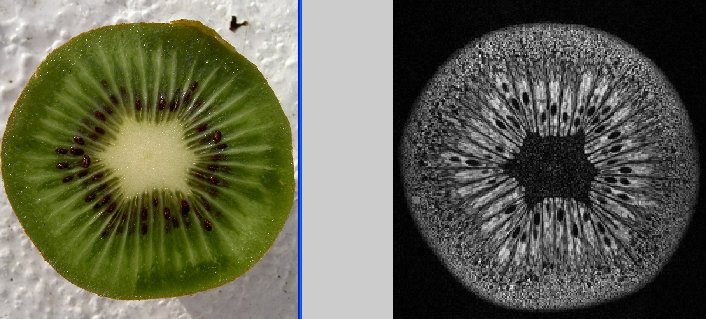
\includegraphics[width=0.78\textwidth]{../../../Lab4-Comp-Imag/Kiwi-challenge/assets/photo_mri_kiwi_20050219.jpg}
\caption{Direct macroscopic comparison from the UiB 2005 dataset: optical cross-section (left) vs.\ 7\,T $T_2$-weighted RARE MRI equatorial slice ($z=64$, $\text{TR}=18.52\text{ s}$, $\text{TE}=63.9\text{ ms}$, right). Notice the striking \textbf{contrast inversion}: the opaque white central \emph{columella} becomes dark in $T_2$ MRI, while translucent watery locular mucilage becomes the brightest tissue in the entire organ.}
\label{fig:kiwi-photo-mri}
\end{figure}

\begin{table}[H]
\centering
\scriptsize
\renewcommand{\arraystretch}{1.18}
\rowcolors{2}{white}{rowalt}
\begin{tabularx}{\textwidth}{L{2.25cm} L{2.3cm} L{3.1cm} L{2.85cm} Y}
\toprule
\rowcolor{uibblue!14}
\textbf{Zone ($r/R$)} & \textbf{Histology ($\mu\text{m}$ scale)} & \textbf{Optical Appearance} & \textbf{7T $T_2$ MRI ($\text{TE}=63.9\text{ ms}$)} & \textbf{Human Clinical Parallel} \\
\midrule
\textbf{1.\ Exocarp} ($0.96\text{--}1.00$) & Suberized periderm + air-filled \emph{trichomes} & Thin brown fuzzy rind & \textbf{Very dark rim} (suberin + air susceptibility dephasing) & Stratum corneum / Glisson's or renal capsule \\
\textbf{2.\ Outer Pericarp} ($0.62\text{--}0.96$) & Dimorphic parenchyma ($500\text{--}800\,\mu\text{m}$ sac cells + starch \emph{amyloplasts}) & Vivid green ($6x$) or gold ($2x/4x$) flesh & \textbf{Medium-bright speckled grey} ($T_2 \approx 68\text{--}95\text{ ms}$) & Renal cortex / glandular organ parenchyma \\
\textbf{3.\ Vascular Bundles} & Outer collateral \& placental \textbf{amphicribral} bundles \cite{guo2013} & Pale pinpoints & Fine dark striations along septa & Portal triads / arcuate renal arterial tree \\
\textbf{4.\ Locular Gel} ($0.24\text{--}0.62$) & Hydrated pectic mucilage hydrogel in $K=33$ chambers & Translucent pale jelly & \textbf{Brightest foreground} ($T_2 \approx 120\text{ ms}$, $190\times$ seed) & CSF / fluid-filled cysts / synovial fluid \\
\textbf{5.\ Mature Seeds} ($0.24\text{--}0.62$) & Lignified sclereid \emph{testa} + dormant dehydrated embryo & Glossy black ovals ($\sim 1.5\text{ mm}^3$) & \textbf{Jet-black voids} ($T_2 \approx 9.5\text{--}14\text{ ms}$) & Cerebral microbleeds, calcifications, MS plaques \\
\textbf{6.\ Columella} ($0.00\text{--}0.24$) & Dense cellulose/pectin fibrous axial core & \textbf{Opaque bright white} (Mie light scattering) & \textbf{Dark central blade} ($T_2 \approx 24\text{ ms}$, bound water!) & White tendons, ligaments, menisci, fibrous scar \\
\bottomrule
\end{tabularx}
\caption{Master multi-scale Rosetta Table from Notebook~\texttt{00a} connecting macroscopic zones, histology, 7\,T MRI physics, and human medicine.}
\label{tab:atlas-rosetta}
\end{table}

\subsection{The Four Physiological Phases (`0--180 DAA`) \& Human Gut MRI Bridge}

Developmental phenology (\texttt{BBCH} scale \cite{richardson2011}) explains why our February 2005 retail-mature fruit ($\sim 150\text{ DAA}$) was the ideal physical window for Lab~4 segmentation:
\begin{enumerate}
    \item \textbf{Phase I (0--55 DAA):} Fertilized ovules secrete auxin/cytokinins driving rapid cell division; hydrated white ovules still have long $T_2$ ($<2\times$ contrast vs.\ gel --- nearly invisible in MRI!).
    \item \textbf{Phase II (55--115 DAA):} Mitosis stops; phloem carbon is polymerized into osmotically silent \textbf{amyloplast starch} (up to $\sim 8\%$ FW, avoiding a $>1.1\text{ MPa}$ osmotic burst --- identical to hepatic glycogen storage), while seed coats lignify and dehydrate ($T_2: 95 \to 14\text{ ms}$).
    \item \textbf{Phase III (115--160 DAA, Harvest):} $\beta$-amylase cleaves starch into soluble glucose, fructose, and sucrose ($6\% \to 14\%$ $^\circ\text{Brix}$), sustaining turgor to $86\text{ cm}^3$ while creating crisp $190\times$ gel-to-seed MRI contrast.
    \item \textbf{Phase IV (160--180+ DAA, Softening):} Autocatalytic ethylene solubilizes cell-wall pectins (firmness drops $80\text{ N} \to <10\text{ N}$) and the cysteine protease \textbf{actinidin} (\texttt{PDB 2ACT}, homolog of human lysosomal cathepsins) peaks.
\end{enumerate}

\begin{infobox}[Full-Circle Clinical Punchline: From 7T Berry MRI to Human Abdominal MRI]
In the Nottingham human gut MRI crossover trial (\cite{wilkinsonsmith2019}) and a multicenter Rome~IV RCT (\cite{gearry2023}), eating two green kiwifruits twice daily significantly increased small-bowel water content and colonic volume measured by clinical $T_1$/$T_2$ abdominal MRI. The \textbf{exact same pectic mucilage osmotic water-trapping and $T_2$ relaxation physics} that makes locular gel glow brightest inside our 2005 7\,T berry scan is measured inside the human gastrointestinal tract!
\end{infobox}

% =====================================================================
% SECTION 4: QUANTITATIVE GROWTH & MORPHOGENESIS LADDER (NB 01)
% =====================================================================
\section{Quantitative Growth \& Morphogenesis Ladder (Notebook \texttt{01})}
\label{sec:morphogenesis}

From the calibrated 2005 7\,T NIfTI volume ($256\times 256\times 128$, voxel $\Delta V = 0.2344\times 0.2344\times 0.5000 = 0.02747\text{ mm}^3$), Notebook~\texttt{01} extracts $V_{\text{MRI}} = 85.97\text{ cm}^3$ (length $52.5\text{ mm}$, equatorial diameter $52.0\text{ mm}$) and recall-calibrated $\widehat{N}_{\text{cal}} \approx 1{,}440$ seeds ($\sim 2.55\%$ volume fraction). We then climb four mathematical rungs to explain how $2.5\%$ of the organ orchestrates the other $97.5\%$.

\subsection{Stage 1 (Algebraic): Seed-Hormone Receptor Saturation \& Axial Allometry}

Assuming fertilized seeds secrete auxin/cytokinins proportionally to $N$ and bind maternal pericarp receptors with dissociation constant $K_N = K_d/\alpha$ \cite{pyke1986}:
\begin{equation}
    V_{\text{fruit}}(N) = V_{\text{basal}} + V_{\max}\,\frac{N}{K_N + N}, \qquad \frac{dV_{\text{fruit}}}{dN} = \frac{V_{\max}\,K_N}{(K_N + N)^2}.
\end{equation}
\textbf{Empirical Check on the 2005 7T Scan:} At $\widehat{N}=1{,}440$, the saturation law predicts \textbf{$86.13\text{ cm}^3$} vs.\ measured \textbf{$85.97\text{ cm}^3$} ($77.4\%$ receptor saturation). Slice-by-slice cross-sectional area $A_{\text{MRI}}(z)$ correlates strongly with local seed density across all interior slices (\textbf{$r = 0.851$, $p = 5.84\times 10^{-30}$}) and jumps to \textbf{$r = 0.944$} inside the seed-bearing core ($z \in [14, 49]\text{ mm}$), matching the pharmacodynamic $E_{\max}/\text{EC}_{50}$ law.

\subsection{Stage 2A (ODEs): Bistable \texttt{XY} Floral Sex Switch (\emph{Shy Girl} vs.\ Carpel Fate)}

Every kiwifruit flower starts bisexual. On male vines (\texttt{XXXXXY}, $I_Y = 1$), Y-linked \emph{Shy Girl} (\texttt{SyGI}, $S(t)$ \cite{akagi2018}) represses cytokinin-driven carpel identity $C(t)$ with Hill cooperativity $n=3$; on female vines (\texttt{XXXXXX}, $I_Y = 0$), positive auto-feedback locks $C(t) \to 2.42$ (explaining DICOM \texttt{PatientSex = F}!):
\begin{equation}
    \frac{dS}{dt} = \alpha_Y I_Y - \delta_S S, \qquad \frac{dC}{dt} = \frac{\beta_{\text{CK}}}{1 + (S/K_S)^n} + \frac{\beta_{\text{auto}}\,C^n}{K_C^n + C^n} - \delta_C C.
\end{equation}
\emph{Human parallel:} At gestation week~6, Y-linked \texttt{SRY}/\texttt{SOX9} executes the exact same bistable switch against female \texttt{WNT4}/$\beta$-catenin.

\subsection{Stage 2B (Coupled ODEs + Bloch $T_2$): Lockhart Expansion \& Starch--Sugar Osmosis}

Irreversible viscoplastic volume expansion occurs only when hydrostatic turgor pressure $P(t)$ exceeds mechanical wall yield threshold $Y = 0.52\text{ MPa}$ \cite{lockhart1965,hall2013}:
\begin{equation}
    \frac{dV}{dt} = \phi(t)\,V\,\max\!\big(0,\, P(t) - Y\big), \qquad P(t) = \Psi_{\text{xylem}} + \kappa_{\text{osm}}\frac{M_{\text{sugar}}(t) + M_0(V)}{V(t)} + \Delta P_{\text{seed}}(N),
\end{equation}
\begin{equation}
    \frac{dM_{\text{starch}}}{dt} = f_{\text{st}}(t)J_{\text{phloem}} - k_{\text{hyd}}(t)M_{\text{starch}}, \qquad \frac{dM_{\text{sugar}}}{dt} = \big(1 - f_{\text{st}}(t)\big)J_{\text{phloem}} + k_{\text{hyd}}(t)M_{\text{starch}} - r_{\text{resp}}M_{\text{sugar}},
\end{equation}
coupled to transverse spin-echo MRI physics $S_{\text{RARE}}(t) \approx \rho\,\exp\!\big(-\text{TE}/T_2(t)\big)$ at $\text{TE}=63.9\text{ ms}$:
\begin{itemize}
    \item \textbf{Volume \& Nonlinear Drought Sensitivity:} Predicts \textbf{$86.86\text{ cm}^3$} at Day~160 ($N=1{,}440$). Because growth depends on \emph{excess} pressure $(P - Y)$, a mild $-0.22\text{ MPa}$ water deficit ($\sim 18\%$ of $P$) slashes final fruit volume by \textbf{$42\%$ ($86.9 \to 50.0\text{ cm}^3$)} --- directly mirroring how a modest arterial pressure drop halts glomerular filtration (\texttt{GFR}) once $P_{\text{GC}}$ approaches $P_{\text{BS}} + \pi_{\text{GC}}$!
    \item \textbf{Emergent 7T Contrast:} Gel/seed RARE ratio grows from \textbf{$1.59\times$} at Day~40 (hydrated white ovules) to \textbf{$190.3\times$} at Day~160 (lignified black seeds vs.\ liquefied mucilage).
\end{itemize}

\subsection{Stage 3 (Spatial PDEs): 1D Turing Ring (\texttt{K = 33}) \& 2D Paracrine Canalization}

\begin{enumerate}
    \item \textbf{Model 3A --- 1D Periodic Schnakenberg Turing PDE ($s \in [0, L)$):}
    \begin{equation}
        \frac{\partial u}{\partial t} = D_u \frac{\partial^2 u}{\partial s^2} + \gamma_{\text{rxn}}\!\left(a - u + u^2 v\right), \qquad \frac{\partial v}{\partial t} = D_v \frac{\partial^2 v}{\partial s^2} + \gamma_{\text{rxn}}\!\left(b - u^2 v\right),
    \end{equation}
    with fast substrate/inhibitor diffusion ($D_v \gg D_u$). Starting from $1.5\%$ random noise around $(u_0, v_0) = (a+b,\, b/(a+b)^2)$, the hexaploid floral ring spontaneously crystallizes into \textbf{$K_{\text{Turing}} = 33$ carpel peaks}, matching the \textbf{$K_{\text{MRI}} = 33$} radial locules counted on equatorial slice $z=64$! (Analytical ploidy proof $2x\to 4x\to 6x$ continues in Part~2.)
    \item \textbf{Model 3B --- 2D Screened-Poisson Paracrine Diffusion ($\ell = \sqrt{D/\gamma}$):}
    \begin{equation}
        \big(\ell^2 \nabla^2 - 1\big) c(x, y) = -\frac{\alpha}{\gamma}\sum_{i=1}^{N_{\text{eq}}} \delta(\mathbf{x} - \mathbf{x}_i), \qquad R_{\text{outer}}(\theta) = R_{\text{core}}(\theta) + g_{\text{basal}} + g_{\max}\frac{\bar{c}(\theta)}{K_c + \bar{c}(\theta)}.
    \end{equation}
    On our 2005 scan, $15^\circ$ radial wedges vary $2.9\times$ in seed count ($14\text{--}41$ seeds), yet outer radius $R_{\text{outer}}(\theta)$ varies by only \textbf{$3.5\%$ ($25.32\text{--}26.23\text{ mm}$)} --- classic \textbf{developmental canalization} via diffusive smoothing + receptor saturation! Blocking pollination on one hemisphere breaks canalization, collapsing $R(\theta)$ into a flat-sided berry ($\Delta R = 9.4\text{ mm}$, $16.98\text{--}26.38\text{ mm}$).
\end{enumerate}

% =====================================================================
% SECTION 5: RECIPES, SELF-CHECK & REFERENCES
% =====================================================================
\section{Minimal Python Recipes, Self-Check Q\&A \& References}

\begin{lstlisting}[style=pybmed]
import numpy as np

def step_turing_ring(u: np.ndarray, v: np.ndarray, Du=0.02, Dv=1.0, a=0.1, b=0.9, gamma=280.0, ds=0.1, dt=1e-4):
    """One explicit periodic-ring step of the 1D Schnakenberg Turing PDE (NB 01 Stage 3A)."""
    lap_u = (np.roll(u, -1) + np.roll(u, 1) - 2.0 * u) / (ds ** 2)
    lap_v = (np.roll(v, -1) + np.roll(v, 1) - 2.0 * v) / (ds ** 2)
    u2v = (u * u) * v
    return u + dt * (Du * lap_u + gamma * (a - u + u2v)), v + dt * (Dv * lap_v + gamma * (b - u2v))
\end{lstlisting}

\begin{qabox}[Check Your Understanding: Why Does a White \emph{Columella} Turn Dark in 7T $T_2$ MRI?]
\textbf{Question:} Optically, the central \emph{columella} is the brightest white structure in a sliced kiwifruit, yet on our 7\,T $T_2$-weighted RARE scan ($\text{TE}=63.9\text{ ms}$) it appears dark grey/black. Why do optical and MRI brightness invert?\\[2pt]
\textbf{Answer:} Optical whiteness arises from \textbf{Mie light scattering} off densely packed cellulose/pectin cell walls and micro-interfaces (like snow or white paper). In $T_2$-weighted MRI, however, water protons tightly bound to dense macromolecules undergo rapid spin--spin dephasing (\textbf{short $T_2 \approx 24\text{ ms}$}), so signal decays before the echo at $\text{TE}=63.9\text{ ms}$ --- the exact reason glistening white human tendons and ligaments look dark on clinical $T_2$ MRI!
\end{qabox}

\begin{thebibliography}{9}
\scriptsize
\setlength{\itemsep}{1.5pt}
    \bibitem{guo2013} Guo X et al. \emph{Anatomical and histological study of kiwifruit vascular and carpel architecture.} \textbf{Frontiers in Plant Science} 4:473 (2013). \href{https://pmc.ncbi.nlm.nih.gov/articles/PMC3797463/}{PMC3797463}
    \bibitem{richardson2011} Richardson AC et al. \emph{Fruit development of the diploid kiwifruit, Actinidia chinensis `Hort16A'.} \textbf{BMC Plant Biology} 11:182 (2011). \href{https://pmc.ncbi.nlm.nih.gov/articles/PMC3261216/}{PMC3261216}
    \bibitem{pyke1986} Pyke NB \& Alspach PA. \emph{Inter-relationships of fruit weight, seed number and seed weight in kiwifruit.} \textbf{N.Z.\ J.\ Agric.\ Res.} 29:471--476 (1986).
    \bibitem{akagi2018} Akagi T et al. \emph{A Y-encoded suppressor of feminization arose via lineage-specific duplication of a cytokinin response regulator in kiwifruit.} \textbf{The Plant Cell} 30:780--795 (2018). \href{https://doi.org/10.1105/tpc.17.00787}{doi:10.1105/tpc.17.00787}
    \bibitem{lockhart1965} Lockhart JA. \emph{An analysis of irreversible plant cell elongation.} \textbf{J.\ Theor.\ Biol.} 8:264--275 (1965).
    \bibitem{hall2013} Hall AJ et al. \emph{A biophysical model of kiwifruit (Actinidia deliciosa) berry development.} \textbf{J.\ Exp.\ Bot.} 64:5473--5483 (2013). \href{https://doi.org/10.1093/jxb/ert317}{doi:10.1093/jxb/ert317}
    \bibitem{turing1952} Turing AM. \emph{The chemical basis of morphogenesis.} \textbf{Phil.\ Trans.\ R.\ Soc.\ Lond.\ B} 237:37--72 (1952). \href{https://doi.org/10.1098/rstb.1952.0012}{doi:10.1098/rstb.1952.0012}
    \bibitem{wilkinsonsmith2019} Wilkinson-Smith V et al. \emph{Mechanisms underlying effects of kiwifruit on intestinal function shown by MRI in healthy volunteers.} \textbf{Aliment.\ Pharmacol.\ Ther.} 49:759--768 (2019). \href{https://pubmed.ncbi.nlm.nih.gov/30706488/}{PMID:30706488}
    \bibitem{gearry2023} Gearry R et al. \emph{Consumption of 2 green kiwifruits daily improves constipation and abdominal comfort --- results of an international multicenter randomized controlled trial.} \textbf{Am.\ J.\ Gastroenterol.} 118:1058--1068 (2023). \href{https://pubmed.ncbi.nlm.nih.gov/36537785/}{PMID:36537785}
\end{thebibliography}

\end{document}
